%%%%%%%%%%%%%%%%%%%%%%%%%%%%%%%%%%%%%%%%%
% Short Sectioned Assignment
% LaTeX Template
% Version 1.0 (5/5/12)
%
% This template has been downloaded from:
% http://www.LaTeXTemplates.com
%
% Original author:
% Frits Wenneker (http://www.howtotex.com)
%
% License:
% CC BY-NC-SA 3.0 (http://creativecommons.org/licenses/by-nc-sa/3.0/)
%
%%%%%%%%%%%%%%%%%%%%%%%%%%%%%%%%%%%%%%%%%

%----------------------------------------------------------------------------------------
%	PACKAGES AND OTHER DOCUMENT CONFIGURATIONS
%----------------------------------------------------------------------------------------

\documentclass[paper=a4, fontsize=11pt]{scrartcl} % A4 paper and 11pt font size

\usepackage[T1]{fontenc} % Use 8-bit encoding that has 256 glyphs
\usepackage{fourier} % Use the Adobe Utopia font for the document - comment this line to return to the LaTeX default
\usepackage[english]{babel} % English language/hyphenation
\usepackage{amsmath,amsfonts,amsthm} % Math packages

\usepackage{lipsum} % Used for inserting dummy 'Lorem ipsum' text into the template

\usepackage{sectsty} % Allows customizing section commands
\allsectionsfont{\centering \normalfont\scshape} % Make all sections centered, the default font and small caps

\usepackage{fancyhdr} % Custom headers and footers

% my packages
\usepackage{commath}
\usepackage{mathtools}
\usepackage{graphicx}
\usepackage{algorithm}
\usepackage[]{algpseudocode}
\DeclarePairedDelimiter{\ceil}{\lceil}{\rceil}
\usepackage{pgfplots}
\pgfplotsset{compat=newest}
\usepackage{hyperref}
\usepackage{enumitem}
\usepackage{subcaption}
\usepackage{multirow}
\usepackage{tkz-graph}
\usepackage{adjustbox}
\usepackage{cancel}

\newlist{filedescription}{description}{2}
\setlist[filedescription]{font=\normalfont\normalcolor\bfseries\itshape}

\newlist{paramdescription}{description}{1}
\setlist[paramdescription]{font=\normalfont\normalcolor\itshape}

\pagestyle{fancyplain} % Makes all pages in the document conform to the custom headers and footers
\fancyhead{} % No page header - if you want one, create it in the same way as the footers below
\fancyfoot[L]{} % Empty left footer
\fancyfoot[C]{} % Empty center footer
\fancyfoot[R]{\thepage} % Page numbering for right footer
\renewcommand{\headrulewidth}{0pt} % Remove header underlines
\renewcommand{\footrulewidth}{0pt} % Remove footer underlines
\setlength{\headheight}{13.6pt} % Customize the height of the header

\numberwithin{equation}{section} % Number equations within sections (i.e. 1.1, 1.2, 2.1, 2.2 instead of 1, 2, 3, 4)
\numberwithin{figure}{section} % Number figures within sections (i.e. 1.1, 1.2, 2.1, 2.2 instead of 1, 2, 3, 4)
\numberwithin{table}{section} % Number tables within sections (i.e. 1.1, 1.2, 2.1, 2.2 instead of 1, 2, 3, 4)

\setlength\parindent{0pt} % Removes all indentation from paragraphs - comment this line for an assignment with lots of text

% new commands
\newcommand{\filename}[1]{\textbf{\textit{#1}}}
\newcommand{\funcname}[1]{\textbf{#1}}
\newcommand{\inv}{^{\raisebox{.2ex}{$\scriptscriptstyle-1$}}}
\renewcommand{\vec}[1]{\mathbf{#1}}

\makeatletter
\renewcommand*\env@matrix[1][*\c@MaxMatrixCols c]{%
  \hskip -\arraycolsep
  \let\@ifnextchar\new@ifnextchar
  \array{#1}}
\makeatother

\makeatletter
\def\BState{\State\hskip-\ALG@thistlm}
\makeatother

\DeclareMathAlphabet{\mathcal}{OMS}{cmsy}{m}{n}
\DeclareMathOperator*{\argmin}{arg\,min} % Jan Hlavacek

%----------------------------------------------------------------------------------------
%	TITLE SECTION
%----------------------------------------------------------------------------------------

\newcommand{\horrule}[1]{\rule{\linewidth}{#1}} % Create horizontal rule command with 1 argument of height

\title{	
\normalfont \normalsize 
\textsc{Mathematical foundations of computer graphics and vision} \\ [25pt] % Your university, school and/or department name(s)
\horrule{0.5pt} \\[0.4cm] % Thin top horizontal rule
\huge Exercise 4. Sampling Patterns and Graph Cuts\\ % The assignment title
\horrule{2pt} \\[0.5cm] % Thick bottom horizontal rule
}

\author{Dongho Kang \\ \small 16-948-598} % Your name

\date{\normalsize May 7, 2017} % Today's date or a custom date

\begin{document}

\maketitle % Print the title

%----------------------------------------------------------------------------------------
%	README
%----------------------------------------------------------------------------------------

MATLAB R2016b version was used for coding and testing:

\begin{center}
MathWorks, MATLAB R2016b (9.1.0.441655) \\
64-bit (maci64) 
\end{center}

The \filename{code} directory contains the followings:

\begin{filedescription}
	\item [part1\_1.m] script .m file for exercise part 1.1.
	\item [part1\_2.m] script .m file for exercise part 1.2.
	\item [part2\_1.m] script .m file for exercise part 2.1. 
	\item [part2\_2.m] script .m file for exercise part 2.2. 
	\item [PART I] provided directory for part 1.
	\item [PART II] directory which contains implementation of part 2 and provided files including skeleton code etc.
	\item [img] directory which contains images for testing part 2.2   
	\item [result] result image of part 1 and part 2.
\end{filedescription}

For running each .m script, check dependencies (especially for \filename{part2\_1.m} and \filename{part2\_2.m}) and adjust parameters first. Note that \textbf{these scripts only work properly in MATLAB R2016b environment} and \textbf{have done in Mac OS 10.11.6.} More details are stated in the \textit{Running} section of each parts.

%----------------------------------------------------------------------------------------
%	PROBLEM 1
%----------------------------------------------------------------------------------------

\section{exercise part 1: Analyzing Sampling Patterns}

In this exercise, two analysis techniques for sampling distributions was implemented:

\begin{enumerate}
	\item Periodogram (task 1)
	\item Pair Correlation Functions (task 2)
\end{enumerate}

%----------------------------------------------------------------------------------------
%	PERIODOGRAMS
%----------------------------------------------------------------------------------------
\subsection{Task 1: Computing periodograms of sampling patterns}

%----------------------------------------------------------------------------------------
\subsubsection{Description}

The periodogram is computed by \textbf{taking the Fourier transform of the impulse process corresponding to the sampling pattern.} It can be estimated by follows:

\begin{equation}
	P(w) = \abs{ \mathcal{F} [\frac{1}{n} \sum_{i=1}^{n} \delta(\vec{x} - \vec{x_i})]}^2
\end{equation}

where $\delta$ is the Dirac delta function, $\vec{x_i}$ are the locations of the points in a given points distribution and $\mathcal{F}$ denotes the Fourier transform. As suggested, this was implemented by rasterizing the function $\frac{1}{n} \sum_{i=1}^{n} \delta(\vec{x} - \vec{x_i})$ and taking the discrete Fourier transform by using MATLAB function \funcname{fft2}. 
\\

The periodogram was generated for the 4 different sampling algorithms, \textit{Matern, FPO, Dart} and \textit{Balzer}. For each algorithm, results from 10 different dataset were averaged.  

%----------------------------------------------------------------------------------------
\subsubsection{Running}

Run the script \filename{part1\_1.m} after setting the parameter \textit{width, height} for width and height of initial image. The default values are 400 for both \textit{width} and \textit{height}.

%----------------------------------------------------------------------------------------
\subsubsection{Result}

The Figure 1.1 is averaged periodograms of different sampling algorithms. In order to get a clear result image, the periodogram was scaled by 200.

\begin{figure}[t]
\caption{Averaged periodograms for the Matern, FPO, Dart and Balzer algorithms\label{fig:simple}}
\noindent\makebox[\textwidth]{
  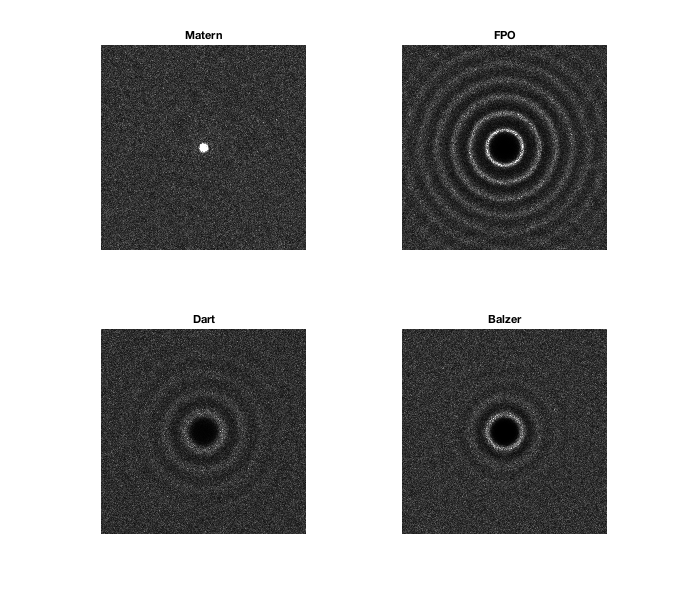
\includegraphics[width=\textwidth]{periodogram-mean.png}
}
\end{figure}

\pagebreak

%----------------------------------------------------------------------------------------
%	PAIR CORRELATION FUNCTION
%----------------------------------------------------------------------------------------
\subsection{Task 2: Computing the pair correlation function of sampling patterns}

%----------------------------------------------------------------------------------------
\subsubsection{Description}

Another way to analyze point distribution is via point process statistics. The pair correlation function (PCF) is widely accepted as the most informative. This measure $g(\vec{x}, \vec{y})$ describes the joint probability of having points at locations $\vec{x}$, and $\vec{y}$ at the same time. 
\\

In the isotropic case, PCF is only depends on the distance between the points and can be estimated as follows:

\begin{equation}
	\hat{g}(r) = \frac{\abs{V}}{\abs{\partial V_d} r^{d-1} n^2} \sum_{i \neq j} k_\sigma (r - d(\vec{x}_i, \vec{x}_j))
\end{equation}

Here $n$ is the number of samples and $\abs{\partial V_d}$ denotes the volume of the boundary of a unit sphere in a $d$ dimensional domain. Since it's 2-dimensional case, $d = 2$, $\abs{V} = 1$, $\abs{\partial V_d} = 2 \pi$ and $d(\vec{x}_i, \vec{x}_j)$ is euclidean distance. The Gaussian kernel was used for $k_\sigma(x) = \frac{1}{\sqrt{\pi} \sigma} e^{-x^2 / \sigma^2}$. For $\sigma$, as suggested in the manual, $\sigma = 0.25$ was used. \\

\textbf{The most tricky part is choosing $r_a$, $r_b$ and normalizing the data}. $r_a$ and $r_b$ are the lower and upper limit of the $r$ values. In order to define these parameters in relative terms, sample points should be normalized by the distance $r_{max}$ defined as the minimum distance between pairs of points for the maximum packing of points in a given volume.\cite{oztireli2012analysis} Two methods can be adapted for determining the $r_{max}$ value as follows:

\begin{itemize}
	\item the method by Lagae and Dutr\'{e} \cite{lagae2008comparison}:
	\begin{equation}
		r_{max} = \sqrt{\frac{1}{2\sqrt{3} N}}
	\end{equation}
	
	where N is the number of samples. For $N = 1024$, $r_{max} = 0.0168$.
	
	\item the method by Gamito and Maddock \cite{gamito2009accurate}: 
	\begin{equation}
		r_{max} = \sqrt[n]{\frac{\gamma_{n_{max}}}{N} \frac{\Gamma(\frac{n}{2} + 1)}{\pi^{n/2}}}
	\end{equation}  
	
	where N is the number of samples, $\Gamma$ denotes Gamma function, $n = 2$, and $\gamma_{n_{max}} = \frac{1}{6} \pi \sqrt{3}$ for 2-dimensional case. In fact, since $\Gamma(2) = 1$ for $n = 2$, $r_{max}$ is exactly same as $r_{max}$ calculated by Lagae and Dutr\'{e} method.
\end{itemize}

\textbf{As normalizing the samples by dividing by $r_{max}$, $\abs{V}$ also should be divided by $r_{max}^2$.} For the best value of $r_a$ and $r_b$, $r_a = 0.01 \sigma$, $r_b = 5$ were suggested but here $r_a = 2 \sigma$, $r_b = 10$ were used because of the numerical issue. 

%----------------------------------------------------------------------------------------
\subsubsection{Running}

Run the script \filename{part1\_2.m} after setting the parameter \textit{array\_size} for the number of $r$ values. Since every parameter was carefully chosen, do not change any value except \textit{array\_size}.

%----------------------------------------------------------------------------------------
\subsubsection{Result}

The Figure 1.2 is PCF of different sampling algorithms. The first datasets (\filename{<algorithm>/1.txt}) for each algorithm were used as sample data.

\begin{figure}[t]
\caption{PCF for the Matern, FPO, Dart and Balzer algorithms\label{fig:simple}}
\noindent\makebox[\textwidth]{
  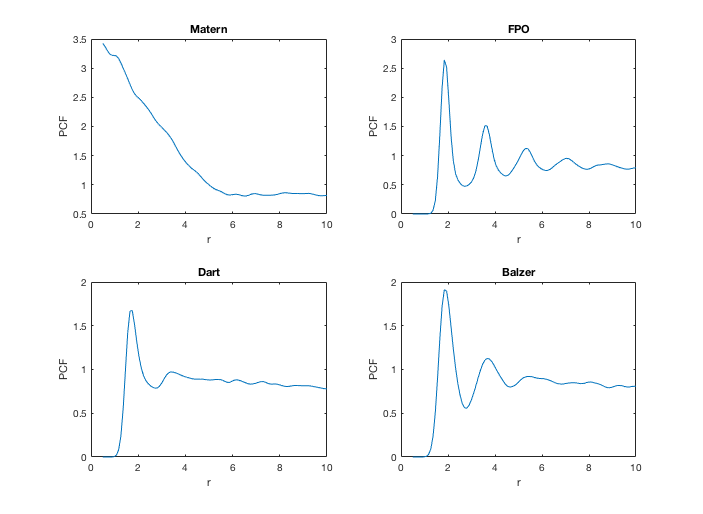
\includegraphics[width=\textwidth]{pcf.png}
}
\end{figure}

\pagebreak

%----------------------------------------------------------------------------------------
%	Discussion
%----------------------------------------------------------------------------------------
\subsection{Discussion}

\begin{itemize}
	\item Why we had to average over multiple point sets for each algorithm when computing the periodograms but not when computing the PCF's? \\
	
	Referring to \cite{oztireli2012analysis}, unlike periodograms, \textbf{the PCF interpretes directly linked to the distribution of the distances between pairs of points} i.e. the PCF, itself is statistical analysis. 
	
	Looking close into equation (1.2), the PCF includes the kernel $k_\sigma (r - d(\vec{x}_i, \vec{x}_j))$ term thus, it's already smoothing (or averaging) the distribution of given sample points. That is why the PCF is called \textbf{smoothed histogram}. 
	
	Besides, the periodogram without averaging is not a statistical analysis. Figure 1.3 is the periodogram which created with one dataset points. Since itself is not statistical, it's hard to find a pattern of each algorithm. Thus in order to find a pattern of certain sampling algorithm, periodogram should be averaged over a number of datasets.   
	
	\begin{figure}[t]
	\caption{The given graphical model for task 1.\label{fig:simple}}
	\noindent\makebox[\textwidth]{
			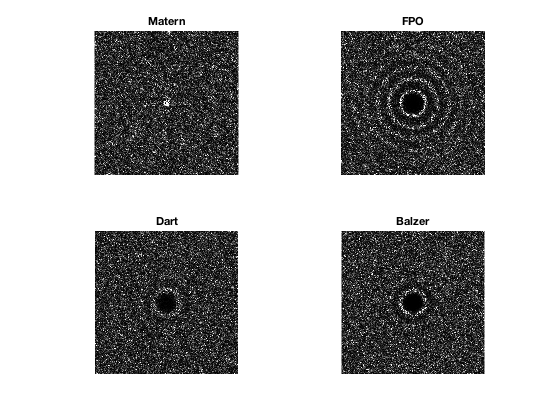
\includegraphics[width=\textwidth]{periodogram-1.png}
	}
	\end{figure}
	
	\pagebreak
	
	\item Is the PCF are sufficient to describe the provided point patterns as they are only one dimensional, while the periodograms are two dimensional? Do the periodograms contain more information for the provided patters? \\
	
	The \cite{oztireli2012analysis} only considered stationary and isotropic case i.e. translation and rotation invariant. Under the assumption, \textbf{the joint probability $g(\vec{x}, \vec{y})$ of having points at location $\vec{x}$ and $\vec{y}$ at the same time only depends on the distance between the points.} Thus, though the PCF is only one dimensional, it can describe the point patterns. \\
	
	However, the PCF is spatial domain analysis while the periodogram is frequency domain analysis. \textbf{Therefore periodogram has more information about certain patterns' properties in frequency domain.}
	
\end{itemize}

\pagebreak

%----------------------------------------------------------------------------------------
%	PROBLEM 2
%----------------------------------------------------------------------------------------

\section{exercise part 2: Interactive Segmentation with Graph Cut}


%----------------------------------------------------------------------------------------
%	Handling max flow
%----------------------------------------------------------------------------------------
\subsection{Task 1: Handling max flow}

\subsubsection{Description}

\begin{figure}[H]
\caption{The given graphical model for task 1.\label{fig:simple}}
\vspace*{5mm}
\centering
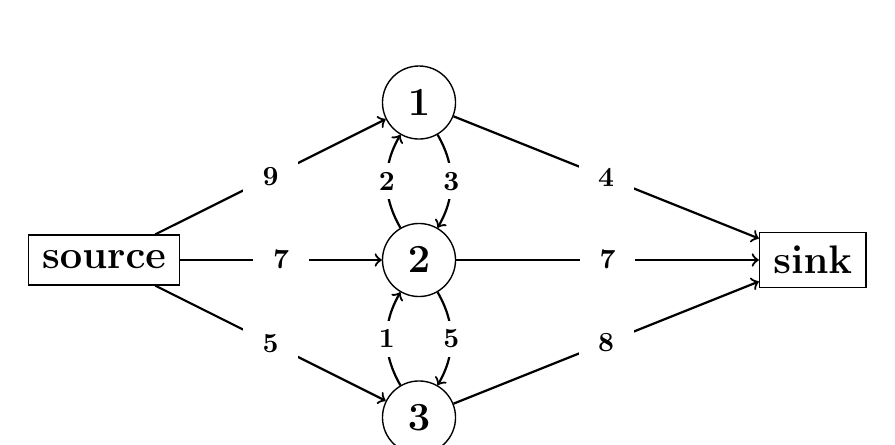
\begin{tikzpicture}
	\GraphInit[vstyle = Dijkstra]
	\tikzset{
	  LabelStyle/.style = { minimum width = 2em, font = \bfseries },
	  VertexStyle/.append style = { inner sep=5pt,
	                                font = \Large\bfseries},
	  EdgeStyle/.append style = {->} }
%	\draw[help lines] (-2, -2) grid (2, 2);
	\SetGraphUnit{2}
	\Vertex{2}
	\begin{scope}[VertexStyle/.append style = {inner sep = 5pt,
                                           shape=rectangle}]
	\EA[unit=5](2){sink}
	\WE[unit=4](2){source}
	\end{scope}
	\NO[unit=2](2){1}
	\SO[unit=2](2){3}
	\Edge[label = 9](source)(1)
	\Edge[label = 7](source)(2)
	\Edge[label = 5](source)(3)
	\Edge[label = 3, style={bend left}](1)(2)
	\Edge[label = 2, style={bend left}](2)(1)
	\Edge[label = 1, style={bend left}](3)(2)
	\Edge[label = 5, style={bend left}](2)(3)
	\Edge[label = 4](1)(sink)
	\Edge[label = 7](2)(sink)
	\Edge[label = 8](3)(sink)
\end{tikzpicture}
\end{figure}

The max flow problem for Figure 2.1 was solved by the algorithm by Boykov and Kolmogorov (BK algorithm). It was implemented using \textit{BK library}. The comparison between the result by the algorithm and the result by hand is discussed in the section 2.1.4.
\\

For unary costs (edges to source and sink) and pairwise costs (edges between nodes), following values were set as input: 

\begin{table}[h]
\captionof{table}{Unary costs for assigning label by BK algorithm} \label{tab:title} 
\centering
\begin{tabular}{| c | c | c | c | }
\hline
label		& node 1 	& node 2	& node 3 \\
\hline 
source (1)	& 4 		& 7			& 8 	 \\ 
\hline							
sink (2)	& 9 		& 7			& 5  	 \\ 
\hline							
\end{tabular}
\end{table}

\textbf{The cost for assigning source(label 1) to node is defined as the cost of cutting the edge between the node and the sink terminal.} For sink(label 2), it's the cost of cutting the edge between the node and the source terminal.  

\begin{table}[h]
\captionof{table}{Pairwise costs between nodes. From row to column. } \label{tab:title} 
\centering
\begin{tabular}{| c | c | c | c | }
\hline
			& node 1 	& node 2	& node 3 \\
\hline 
node 1		& . 		& 3			& . 	 \\ 
\hline							
node 2		& 2 		& .			& 5  	 \\ 
\hline
node 3		& .			& 1			& .		\\
\hline							
\end{tabular}
\end{table}


%----------------------------------------------------------------------------------------
\subsubsection{Running}

Since third party library \textit{BK library} was used, check if the library was built properly. All library files including \filename{bin} directory which contains the compiled binaries, should be placed in the \filename{PART II/GraphCut} directory. \\

Run the script \filename{part2\_1.m}. The script invoke subscript \filename{PART II/task1.m}, the implementation of computing max flow of Figure 2.1. 

%----------------------------------------------------------------------------------------
\subsubsection{Result}

The result of the max flow by BK algorithm as follows:

\begin{figure}[H]
\caption{The given graphical model for task 1.\label{fig:simple}}
\vspace*{5mm}
\centering
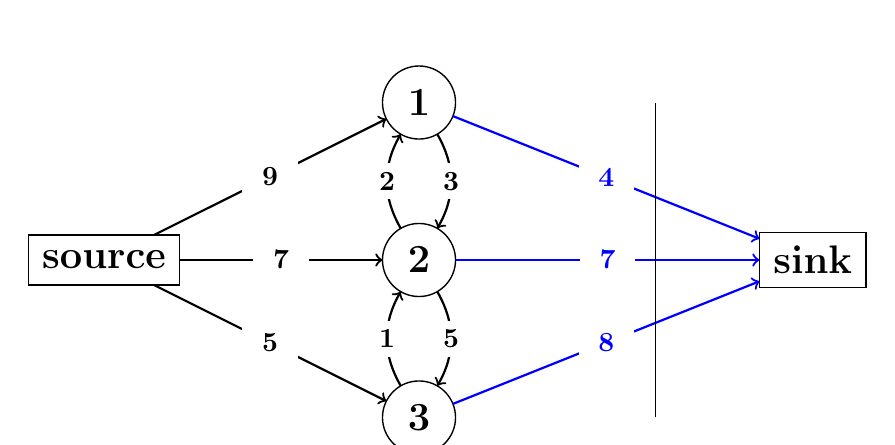
\begin{tikzpicture}
	\tikzset{
	  LabelStyle/.style = { minimum width = 2em, font = \bfseries },
	  VertexStyle/.append style = { inner sep=5pt,
	                                font = \Large\bfseries},
	  EdgeStyle/.append style = {->} }
	\SetGraphUnit{2}
	\Vertex{2}
	\begin{scope}[VertexStyle/.append style = {inner sep = 5pt,
                                           shape=rectangle}]
	\EA[unit=5](2){sink}
	\WE[unit=4](2){source}
	\end{scope}
	\NO[unit=2](2){1}
	\SO[unit=2](2){3}
	\Edge[label = 9](source)(1)
	\Edge[label = 7](source)(2)
	\Edge[label = 5](source)(3)
	\Edge[label = 3, style={bend left}](1)(2)
	\Edge[label = 2, style={bend left}](2)(1)
	\Edge[label = 1, style={bend left}](3)(2)
	\Edge[label = 5, style={bend left}](2)(3)
	\Edge[label = 4, style={blue}, labeltext=blue](1)(sink)
	\Edge[label = 7, style={blue}, labeltext=blue](2)(sink)
	\Edge[label = 8, style={blue}, labeltext=blue](3)(sink)
	\draw (3,-2) -- (3,2);
\end{tikzpicture}
\end{figure}

\begin{itemize}
	\item max flow (or min cut energy) $= 19$ 
	\item label 1 was assigned to all nodes i.e. nodes are connected with source. 
\end{itemize}

\pagebreak

%----------------------------------------------------------------------------------------
\subsubsection{Discussion}

Steps for computing max flow by hand is as follows:

\begin{figure}[H]
\caption{The given graphical model for task 1.\label{fig:simple}}
\vspace*{5mm}
\centering
\begin{subfigure}[b]{0.4\textwidth}
	\begin{adjustbox}{width=\textwidth}
		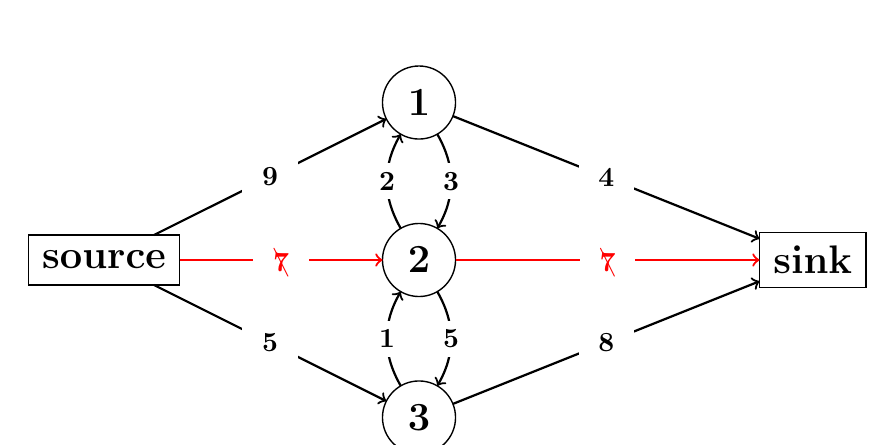
\begin{tikzpicture}
%			\GraphInit[vstyle = Dijkstra]
			\tikzset{
			  LabelStyle/.style = { minimum width = 2em, font = \bfseries },
			  VertexStyle/.append style = { inner sep=5pt,
			                                font = \Large\bfseries},
			  EdgeStyle/.append style = {->} }
			\SetGraphUnit{2}
			\Vertex{2}
			\begin{scope}[VertexStyle/.append style = {inner sep = 5pt,
		                                           shape=rectangle}]
			\EA[unit=5](2){sink}
			\WE[unit=4](2){source}
			\end{scope}
			\NO[unit=2](2){1}
			\SO[unit=2](2){3}
			\Edge[label = 9](source)(1)
			\Edge[label = \bcancel{7}, style=red, labeltext=red](source)(2)
			\Edge[label = 5](source)(3)
			\Edge[label = 3, style={bend left}](1)(2)
			\Edge[label = 2, style={bend left}](2)(1)
			\Edge[label = 1, style={bend left}](3)(2)
			\Edge[label = 5, style={bend left}](2)(3)
			\Edge[label = 4](1)(sink)
			\Edge[label = \bcancel{7}, style=red, labeltext=red](2)(sink)
			\Edge[label = 8](3)(sink)
		\end{tikzpicture}
	\end{adjustbox}	
	\caption{flow $= 7$}
\end{subfigure}
\vspace*{10mm}
\hspace*{10mm}
\begin{subfigure}[b]{0.4\textwidth}
	\begin{adjustbox}{width=1.0\textwidth}
		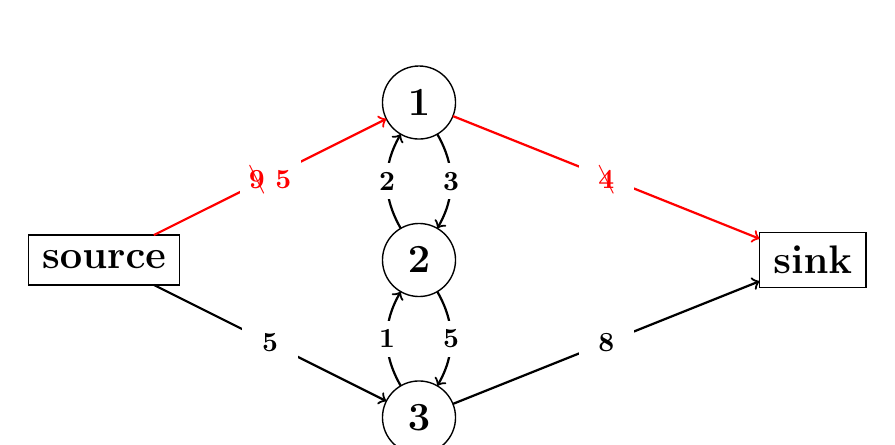
\begin{tikzpicture}
%			\GraphInit[vstyle = Dijkstra]
			\tikzset{
			  LabelStyle/.style = { minimum width = 2em, font = \bfseries },
			  VertexStyle/.append style = { inner sep=5pt,
			                                font = \Large\bfseries},
			  EdgeStyle/.append style = {->} }
			\SetGraphUnit{2}
			\Vertex{2}
			\begin{scope}[VertexStyle/.append style = {inner sep = 5pt,
		                                           shape=rectangle}]
			\EA[unit=5](2){sink}
			\WE[unit=4](2){source}
			\end{scope}
			\NO[unit=2](2){1}
			\SO[unit=2](2){3}
			\Edge[label = \bcancel{9} 5, style=red, labeltext=red](source)(1)
			\Edge[label = 5](source)(3)
			\Edge[label = 3, style={bend left}](1)(2)
			\Edge[label = 2, style={bend left}](2)(1)
			\Edge[label = 1, style={bend left}](3)(2)
			\Edge[label = 5, style={bend left}](2)(3)
			\Edge[label = \bcancel{4}, style=red, labeltext=red](1)(sink)
			\Edge[label = 8](3)(sink)
		\end{tikzpicture}
	\end{adjustbox}	
	\caption{flow $= 11$}
\end{subfigure}
\begin{subfigure}[b]{0.4\textwidth}
	\begin{adjustbox}{width=\textwidth}
		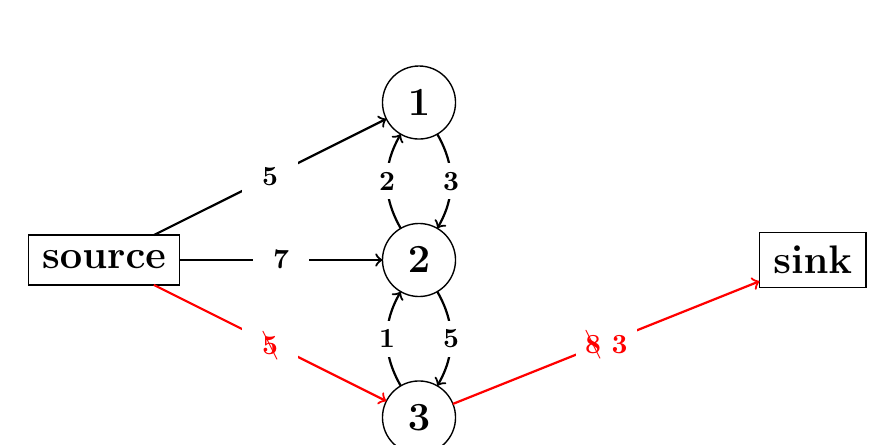
\begin{tikzpicture}
%			\GraphInit[vstyle = Dijkstra]
			\tikzset{
			  LabelStyle/.style = { minimum width = 2em, font = \bfseries },
			  VertexStyle/.append style = { inner sep=5pt,
			                                font = \Large\bfseries},
			  EdgeStyle/.append style = {->} }
			\SetGraphUnit{2}
			\Vertex{2}
			\begin{scope}[VertexStyle/.append style = {inner sep = 5pt,
		                                           shape=rectangle}]
			\EA[unit=5](2){sink}
			\WE[unit=4](2){source}
			\end{scope}
			\NO[unit=2](2){1}
			\SO[unit=2](2){3}
			\Edge[label = 5](source)(1)
			\Edge[label = 7](source)(2)
			\Edge[label = \bcancel{5}, style=red, labeltext=red](source)(3)
			\Edge[label = 3, style={bend left}](1)(2)
			\Edge[label = 2, style={bend left}](2)(1)
			\Edge[label = 1, style={bend left}](3)(2)
			\Edge[label = 5, style={bend left}](2)(3)
			\Edge[label = \bcancel{8} 3, style=red, labeltext=red](3)(sink)
		\end{tikzpicture}
	\end{adjustbox}	
	\caption{flow $= 16$}
\end{subfigure}
\vspace*{10mm}
\hspace*{10mm}
\begin{subfigure}[b]{0.4\textwidth}
	\begin{adjustbox}{width=1.0\textwidth}
		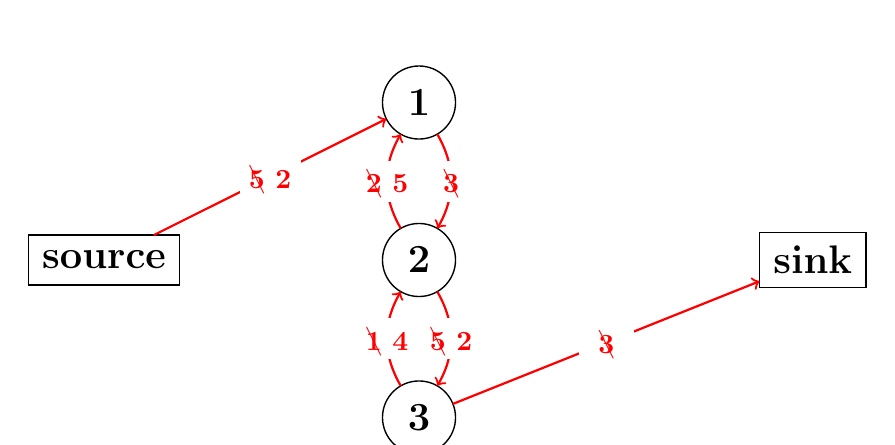
\begin{tikzpicture}
%			\GraphInit[vstyle = Dijkstra]
			\tikzset{
			  LabelStyle/.style = { minimum width = 2em, font = \bfseries },
			  VertexStyle/.append style = { inner sep=5pt,
			                                font = \Large\bfseries},
			  EdgeStyle/.append style = {->} }
			\SetGraphUnit{2}
			\Vertex{2}
			\begin{scope}[VertexStyle/.append style = {inner sep = 5pt,
		                                           shape=rectangle}]
			\EA[unit=5](2){sink}
			\WE[unit=4](2){source}
			\end{scope}
			\NO[unit=2](2){1}
			\SO[unit=2](2){3}
			\Edge[label = \bcancel{5} 2, style=red, labeltext=red](source)(1)
			\Edge[label = \bcancel{3}, style={red, bend left}, labeltext=red](1)(2)
			\Edge[label = \bcancel{2} 5, style={red, bend left}, labeltext=red](2)(1)
			\Edge[label = \bcancel{1} 4, style={red, bend left}, labeltext=red](3)(2)
			\Edge[label = \bcancel{5} 2, style={red, bend left}, labeltext=red](2)(3)
			\Edge[label = \bcancel{3}, style=red, labeltext=red](3)(sink)
		\end{tikzpicture}
	\end{adjustbox}	
	\caption{flow $= 19$}
\end{subfigure}
\begin{subfigure}[b]{0.4\textwidth}
	\begin{adjustbox}{width=\textwidth}
		\begin{tikzpicture}
%			\GraphInit[vstyle = Dijkstra]
			\tikzset{
			  LabelStyle/.style = { minimum width = 2em, font = \bfseries },
			  VertexStyle/.append style = { inner sep=5pt,
			                                font = \Large\bfseries},
			  EdgeStyle/.append style = {->} }
			\SetGraphUnit{2}
			\Vertex{2}
			\begin{scope}[VertexStyle/.append style = {inner sep = 5pt,
		                                           shape=rectangle}]
			\EA[unit=5](2){sink}
			\WE[unit=4](2){source}
			\end{scope}
			\NO[unit=2](2){1}
			\SO[unit=2](2){3}
			\Edge[label = 2](source)(1)
			\Edge[label = 5, style={bend left}](2)(1)
			\Edge[label = 4, style={bend left}](3)(2)
			\Edge[label = 2, style={bend left}](2)(3)
		\end{tikzpicture}
	\end{adjustbox}	
	\caption{terminated with flow $= 19$}
\end{subfigure}
\vspace*{10mm}
\hspace*{10mm}
\begin{subfigure}[b]{0.4\textwidth}
	\begin{adjustbox}{width=1.0\textwidth}
		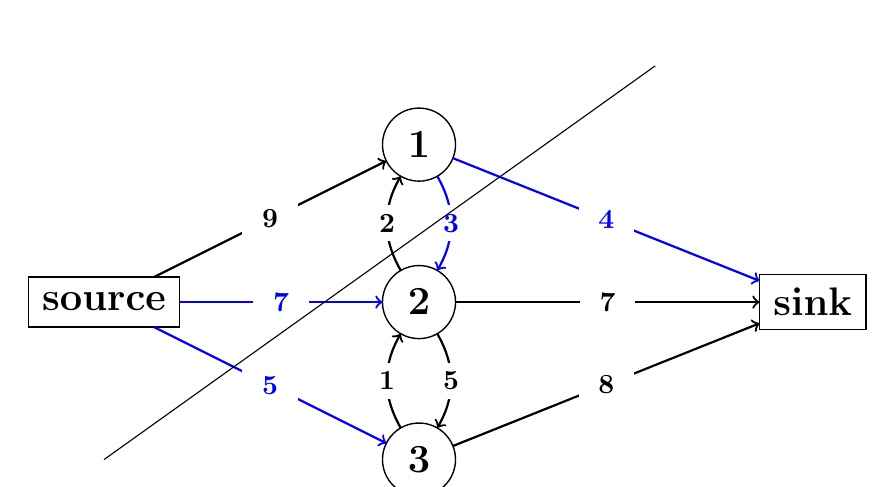
\begin{tikzpicture}
%			\GraphInit[vstyle = Dijkstra]
			\tikzset{
			  LabelStyle/.style = { minimum width = 2em, font = \bfseries },
			  VertexStyle/.append style = { inner sep=5pt,
			                                font = \Large\bfseries},
			  EdgeStyle/.append style = {->} }
			\SetGraphUnit{2}
			\Vertex{2}
			\begin{scope}[VertexStyle/.append style = {inner sep = 5pt,
		                                           shape=rectangle}]
			\EA[unit=5](2){sink}
			\WE[unit=4](2){source}
			\end{scope}
			\NO[unit=2](2){1}
			\SO[unit=2](2){3}
			\Edge[label = 9](source)(1)
			\Edge[label = 7, style={blue}, labeltext=blue](source)(2)
			\Edge[label = 5, style={blue}, labeltext=blue](source)(3)
			\Edge[label = 3, style={bend left, blue}, labeltext=blue](1)(2)
			\Edge[label = 2, style={bend left}](2)(1)
			\Edge[label = 1, style={bend left}](3)(2)
			\Edge[label = 5, style={bend left}](2)(3)
			\Edge[label = 4, style={blue}, labeltext=blue](1)(sink)
			\Edge[label = 7](2)(sink)
			\Edge[label = 8](3)(sink)
			\draw (-4,-2) -- (3,3);
		\end{tikzpicture}
	\end{adjustbox}	
	\caption{graph cut with cost $= 19$}
\end{subfigure}
\end{figure}

\begin{itemize}
	\item max flow (or min cut energy) $= 19$ 
	\item label 1 was assigned to node 1. Thus, node 1 is connected with source. 
	\item label 2 was assigned to node 2 and node 3. Thus, node 2 and node 3 are connected with sink. 
\end{itemize}

The result above is same in max flow with the result by BK algorithm but different in labelling. Both labelling is correct because costs of cutting are 19 in both cases.


%----------------------------------------------------------------------------------------
%	Interactive Segmentation
%----------------------------------------------------------------------------------------
\subsection{Task 2: Interactive Segmentation}

\subsubsection{Description}

An interactive segmentation algorithm was implemented. The steps are as follows:

\begin{enumerate}
	\item Build a color histogram. 
	\item Get unary cost.
	\item Get pairwise cost.
	\item Build and solve a graph. Produce segmentation images. 
	\item Change background using the obtained segmentation. 
\end{enumerate}

The unary and pairwise costs was defined as the definition on \cite{boykov2001interactive}.

\paragraph{Color histogram}

A color histogram of dimension $32 \times 32 \times 32$ was built by a given data which user assigned as foreground or background. Each pixel of image goes to a bin which corresponds to its R, G, B values. For proper generalization, resolution for R, G, B set to 32. Thus, index of bin for a pixel with $I = (r, g, b)$ determined as follows:

\begin{equation}
	\begin{split}
		i_1 &= Q(r, 8) + 1 \\
		i_2 &= Q(g, 8) + 1 \\
		i_3 &= Q(b, 8) + 1 	
	\end{split}
\end{equation}

where $Q(a, b)$ is quotient of dividend $a$ and divisor $b$ and $\vec{i} = (i_1, i_2, i_3)$ is a index of a histogram bin. In order to using the color histogram as probability distribution, it was smoothed and normalized. 

\begin{figure}[b]
	\caption{Color histogram of JCVD.jpg \label{fig:simple}}
	\centering
	\begin{subfigure}[b]{0.4\textwidth}
		\noindent\makebox[\textwidth]{
		  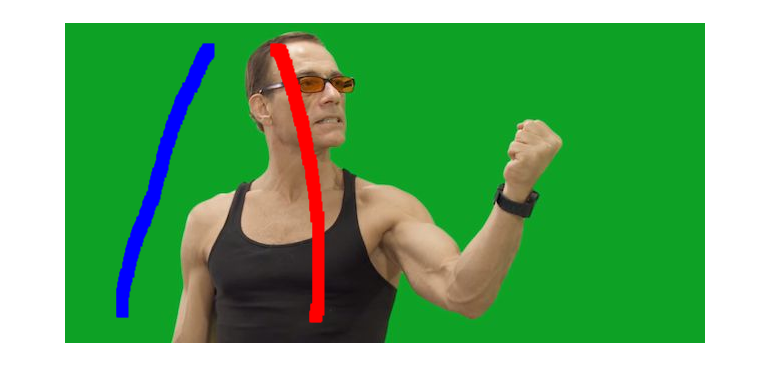
\includegraphics[width=\textwidth]{JCVD.png}
		}
	\caption{JCVD.jpg}
	\end{subfigure}
	\begin{subfigure}[b]{0.25\textwidth}
		\noindent\makebox[\textwidth]{
		  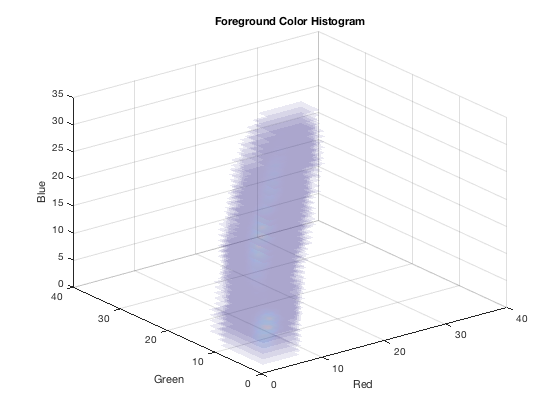
\includegraphics[width=\textwidth]{JCVD-obj-color-histogram.png}
		}
	\caption{foreground}
	\end{subfigure}
	\begin{subfigure}[b]{0.25\textwidth}
		\noindent\makebox[\textwidth]{
		  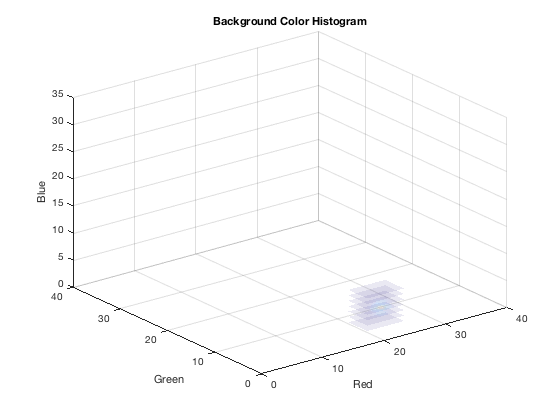
\includegraphics[width=\textwidth]{JCVD-bkg-color-histogram.png}
		}
	\caption{background}
	\end{subfigure}
\end{figure}

\paragraph{Unary cost}

Using color histogram, unary cost for each pixel was calculated:

\begin{table}[H]
\captionof{table}{Definition of unary cost} \label{tab:title} 
\centering
\begin{tabular}{| c | c | c | c | }
\hline
edge						& label						& weight 								& for	\\
\hline 
\multirow{3}{*}{$\{p, S\}$}	& \multirow{3}{*}{$\{ p, T\}$} 	& $\lambda \cdot R_p(\text{"bkg"})$		& $p \in \mathcal{P}, p \notin \mathcal{O} \cup\mathcal{B}$ \\ \cline{3-4}
							&								& K										& $p \in \mathcal{O}$ \\ \cline{3-4}
							&								& 0										& $p \in \mathcal{B}$ \\ \hline	
\multirow{3}{*}{$\{p, T\}$}	& \multirow{3}{*}{$\{ p, S\}$} 	& $\lambda \cdot R_p(\text{"obj"})$		& $p \in \mathcal{P}, p \notin \mathcal{O} \cup\mathcal{B}$ \\ \cline{3-4}
							&								& 0										& $p \in \mathcal{O}$ \\ \cline{3-4}
							&								& K										& $p \in \mathcal{B}$ \\ \hline	
\end{tabular}
\end{table}

$\mathcal{P}$ is a set of pixels. The subsets $\mathcal{O} \subset \mathcal{P}$ and $\mathcal{O} \subset \mathcal{P}$ denote the subsets of pixels marked as "object" and "background" and $\mathcal{O} \cap \mathcal{O} = \emptyset$. \\

Regional penalites $R_p(\cdot)$ is defined as negative log-likelihoods:

\begin{equation}
	\begin{split}
		R_p(\text{"obj"}) &= - \text{ln Pr}(I_p | \mathcal{O}) \\
		R_p(\text{"bkg"}) &= - \text{ln Pr}(I_p | \mathcal{B}) 	
	\end{split}
\end{equation}

where Pr$(I_p | \mathcal{O})$ and Pr$(I_p | \mathcal{O})$ are intensity distributions from the color histogram. For $K$, $K = \infty$ was used. As defining unary cost in the above manner, Figure 2.7 was obtained. (a) is cost of assigning "obj" label to each pixel node (thus the cutting edge cost between node and sink) and (b) is cost of assigning "bkg" label to each pixel node. For each color map, blue indicates low cost and yellow indicates high cost. 

\begin{figure}[H]
	\caption{The unary cost of JCVD.png ($\lambda = 1.0$)\label{fig:simple}}
	\centering
	\begin{subfigure}[b]{0.45\textwidth}
		\noindent\makebox[\textwidth]{
		  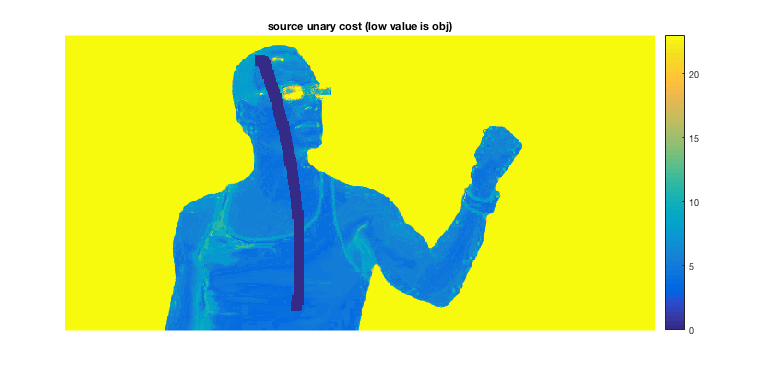
\includegraphics[width=\textwidth]{JCVD-sourcecost-lambda-1.png}
		}
	\caption{source unary cost (blue is obj)}
	\end{subfigure}
	\begin{subfigure}[b]{0.45\textwidth}
		\noindent\makebox[\textwidth]{
		  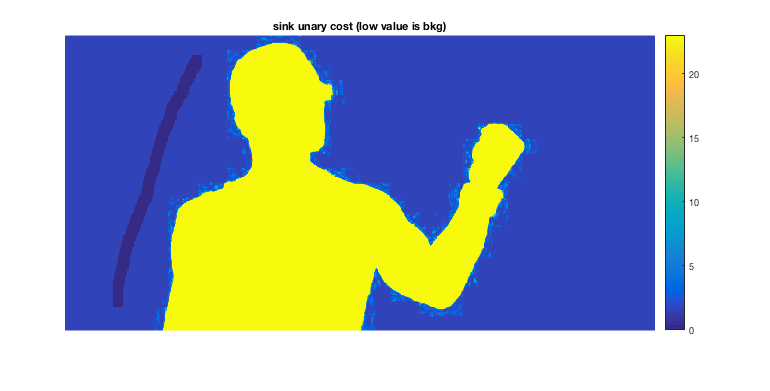
\includegraphics[width=\textwidth]{JCVD-sinkcost-lambda-1.png}
		}
	\caption{sink unary cost (blue is bkg)}
	\end{subfigure}
\end{figure}

\paragraph{Pairwise cost}

Pairwise cost between a pixel and its neighboring 8 pixels was defined as follows:

\begin{table}[H]
\captionof{table}{Definition of pairwise cost} \label{tab:title} 
\centering
\begin{tabular}{| c | c | c | c | }
\hline
edge			& weight 			& for							\\ \hline 
$\{ p, q\}$		& $B_{\{ p, q\}}$	& $\{ p, q\} \in \mathcal{N}$	\\ \hline	
\end{tabular}
\end{table}

where an \textit{ad-hoc} function was used as the boundary penalty $B_{\{ p,q\}}$:

\begin{equation}
	B_{\{ p,q\}} \propto exp\Big( - \frac{(I_p - I_q)^2}{2\sigma^2} \Big) \cdot \frac{1}{dist(p,q)}
\end{equation}

Here, $\sigma = 5$ and the euclidean distance was used for $dist(p,q)$.

\paragraph{Graph and segmentation}

Using BK library, label for each pixel and cost of graph cut was obtained. Figure 2.9 shows the result of graph cut with $lambda = 1.0$ which was applied to JCVD.png. Yellow pixels are assigned to "bkg" label and blues are assigned to "obj".

\begin{figure}[H]
\caption{The label obtained by a graph cut. ($\lambda = 1.0$)\label{fig:simple}}
\centering
	\noindent\makebox[\textwidth]{
			
\includegraphics[width=0.8\textwidth]{JCVD-labels-lambda-1.png}
	}
\end{figure}

%\vspace*{-10mm}
\paragraph{Changing background}

As image segmented into two sets, object("obj") set and background("bkg") set, background pixels can be replaced with a new background image. 

\begin{figure}[H]
\caption{Background change for JCVD.png ($\lambda = 1.0$)\label{fig:simple}}
\centering
	\noindent\makebox[\textwidth]{
			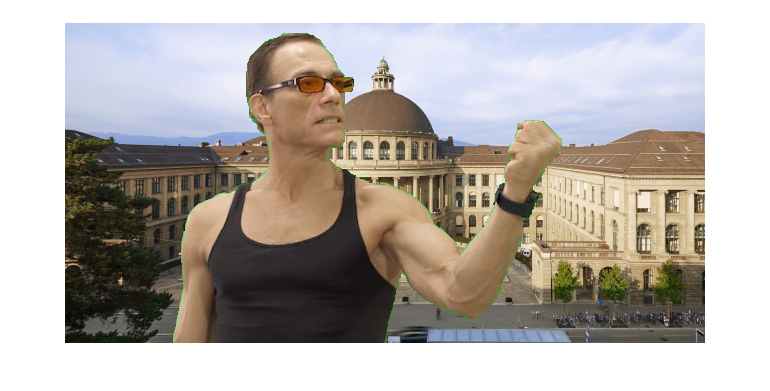
\includegraphics[width=0.8\textwidth]{JCVD-eth-lambda-1.png}
	}
\end{figure}


%----------------------------------------------------------------------------------------
\subsubsection{Running}

Since third party library \textit{BK library} was used, check if the library was built properly. All library files including \filename{bin} directory which contains the compiled binaries, should be placed in the \filename{PART II/GraphCut} directory. \\

Run the script \filename{part2\_2.m}. The script invoke subscript \filename{PART II/interactiveGraphCut.m} which is for GUI windows. Follow the steps below:

\begin{enumerate}
	\item Open an image file.
	\item To change the background, open background image file. (can be skipped)
	\item Indicate foreground and background by red/blue marker. Pre-generated scribbles can be loaded for \filename{JCVD.jpg} and \filename{bat.jpg}.
	\item Enter the value of $\lambda$.
	\item Press the segment button. 
\end{enumerate}

%----------------------------------------------------------------------------------------
\subsubsection{Result}

Image segmentation was tried with different values of the unary cost parameter $\lambda$.

\begin{figure}[H]
	\caption{Image segmentation of JCVD.jpg with different $\lambda$\label{fig:simple}}
	\centering
	\begin{subfigure}[b]{0.45\textwidth}
		\noindent\makebox[\textwidth]{
		  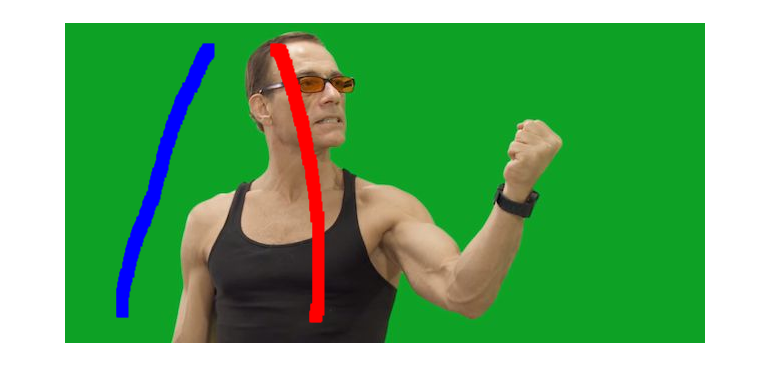
\includegraphics[width=\textwidth]{JCVD.png}
		}
	\caption{JCVD.jpg}
	\end{subfigure}
	\begin{subfigure}[b]{0.45\textwidth}
		\noindent\makebox[\textwidth]{
		  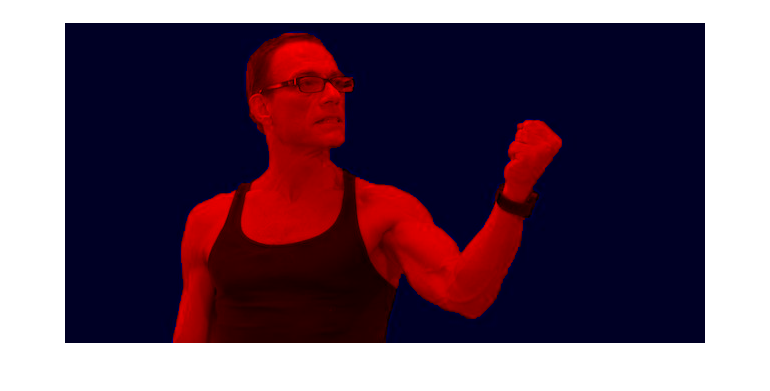
\includegraphics[width=\textwidth]{JCVD-lambda-1.png}
		}
	\caption{$\lambda = 1.0$}
	\end{subfigure}
	\begin{subfigure}[b]{0.45\textwidth}
		\noindent\makebox[\textwidth]{
		  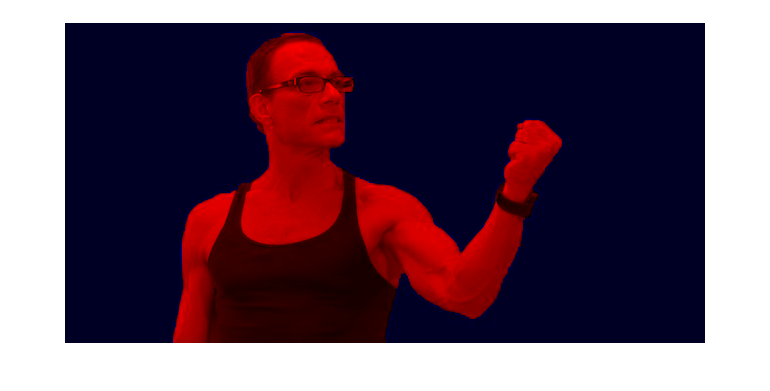
\includegraphics[width=\textwidth]{JCVD-lambda-1e-4.png}
		}
	\caption{$\lambda = 10^{-4}$}
	\end{subfigure}
	\begin{subfigure}[b]{0.45\textwidth}
		\noindent\makebox[\textwidth]{
		  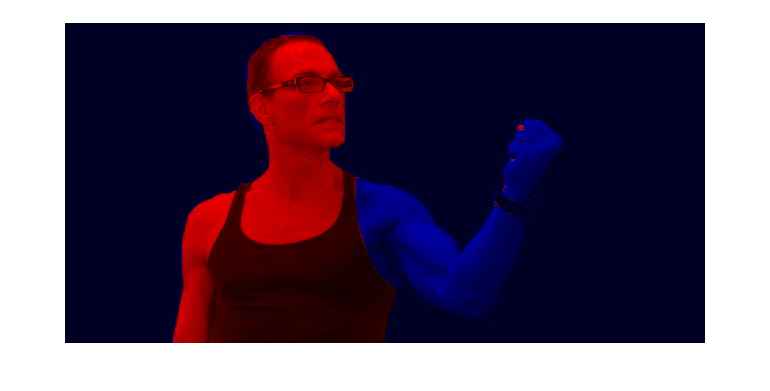
\includegraphics[width=\textwidth]{JCVD-lambda-1e-8.png}
		}
	\caption{$\lambda = 10^{-8}$}
	\end{subfigure}
\end{figure}

\begin{figure}[H]
	\caption{Image segmentation of JCVD.png with different $\lambda$\label{fig:simple}}
	\centering
	\begin{subfigure}[b]{0.45\textwidth}
		\noindent\makebox[\textwidth]{
		  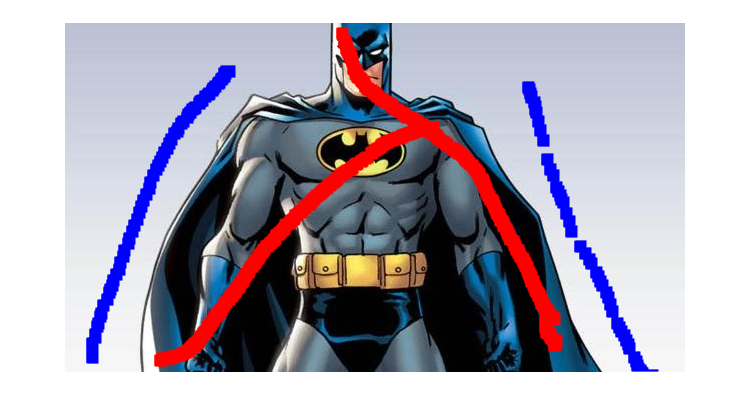
\includegraphics[width=\textwidth]{batman.png}
		}
	\caption{batman.jpg}
	\end{subfigure}
	\begin{subfigure}[b]{0.45\textwidth}
		\noindent\makebox[\textwidth]{
		  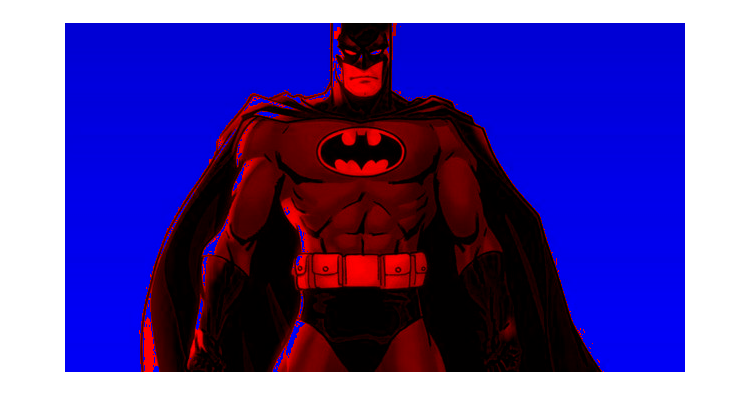
\includegraphics[width=\textwidth]{batman-lambda-1.png}
		}
	\vspace*{-5mm}
	\caption{$\lambda = 1.0$ (the best)}
	\end{subfigure}
	\begin{subfigure}[b]{0.45\textwidth}
		\noindent\makebox[\textwidth]{
		  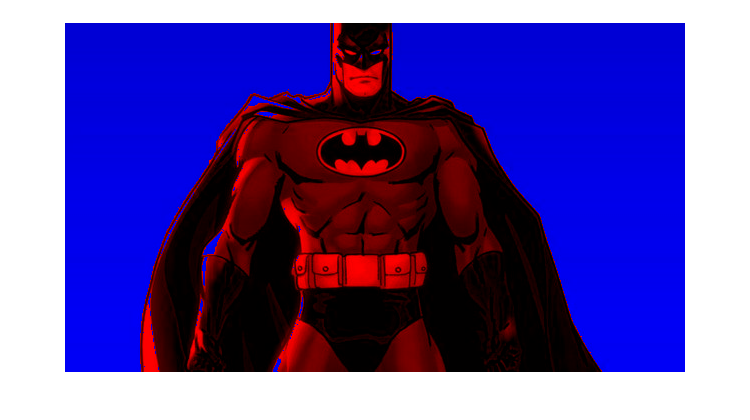
\includegraphics[width=\textwidth]{batman-lambda-2e-3.png}
		}
	\caption{$\lambda = 0.002$}
	\end{subfigure}
	\begin{subfigure}[b]{0.45\textwidth}
		\noindent\makebox[\textwidth]{
		  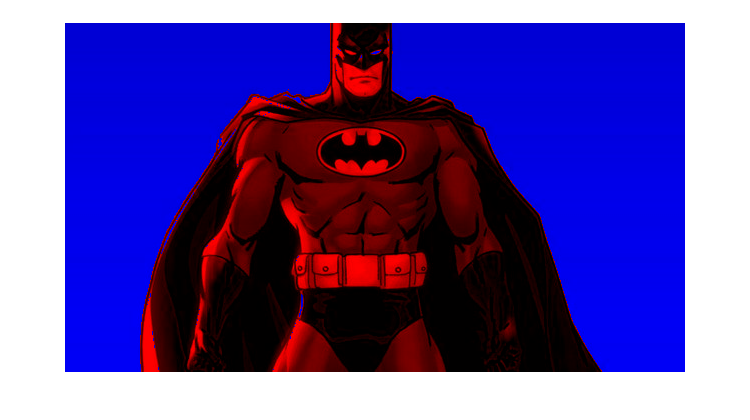
\includegraphics[width=\textwidth]{batman-lambda-1e-6.png}
		}
	\caption{$\lambda = 10^{-6}$ (the best)}
	\end{subfigure}
\end{figure}

The result of changing background is as follows:

\begin{figure}[H]
	\caption{Background change with $\lambda = 1$\label{fig:simple}}
	\centering
	\begin{subfigure}[b]{0.45\textwidth}
		\noindent\makebox[\textwidth]{
		  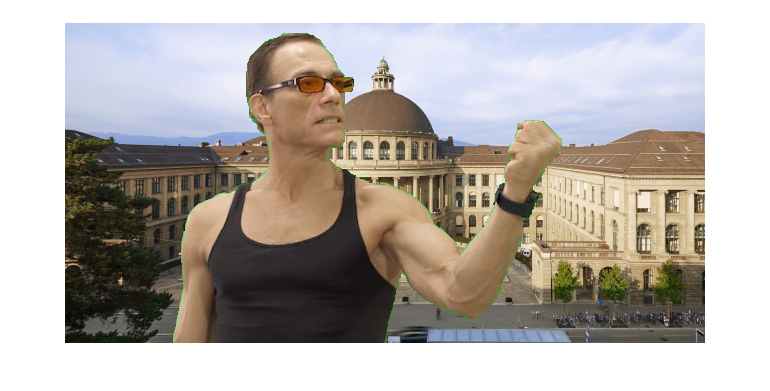
\includegraphics[width=\textwidth]{JCVD-eth-lambda-1.png}
		}
	\caption{Van Damme at ETH}
	\end{subfigure}
	\begin{subfigure}[b]{0.45\textwidth}
		\noindent\makebox[\textwidth]{
		  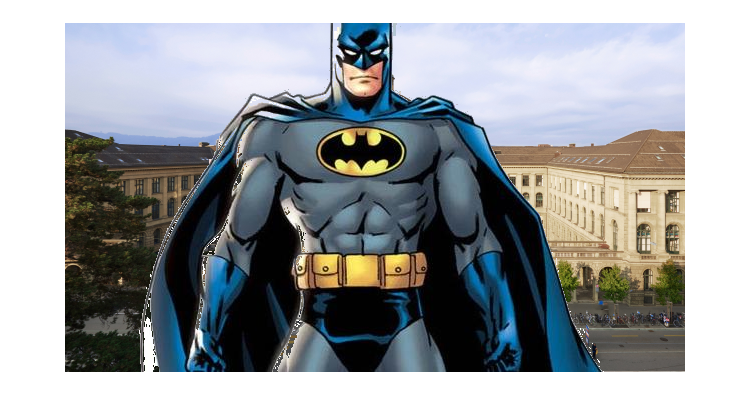
\includegraphics[width=\textwidth]{batman-eth-lambda-1.png}
		}
	\caption{Dark knight at ETH}
	\end{subfigure}
\end{figure}

\pagebreak

Finally, image segmentation was applied to an image which was carefully chosen:

\begin{figure}[H]
	\caption{Image segmentation of JCVD.png with different $\lambda$\label{fig:simple}}
	\centering
	\begin{subfigure}[b]{0.3\textwidth}
		\noindent\makebox[\textwidth]{
		  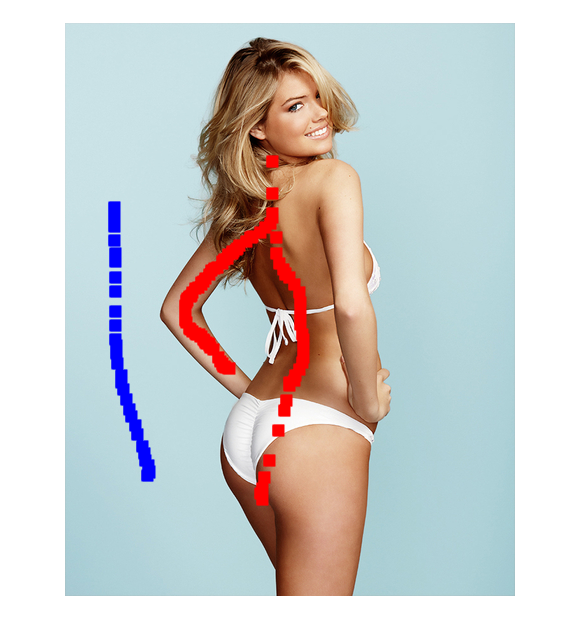
\includegraphics[width=\textwidth]{upton.png}
		}
	\caption{upton.jpg}
	\end{subfigure}
	\begin{subfigure}[b]{0.3\textwidth}
		\noindent\makebox[\textwidth]{
		  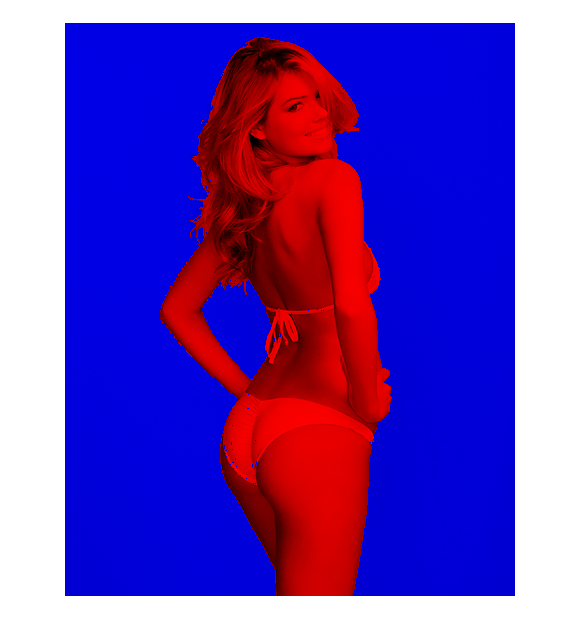
\includegraphics[width=\textwidth]{upton-lambda-1.png}
		}
	\caption{upton.png ($\lambda = 1$)}
	\end{subfigure}
	\begin{subfigure}[b]{0.3\textwidth}
		\noindent\makebox[\textwidth]{
		  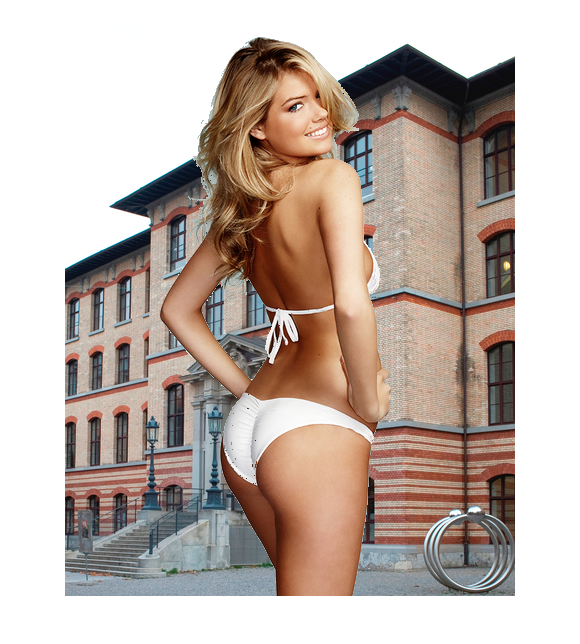
\includegraphics[width=\textwidth]{upton-cab-lambda-1.png}
		}
	\caption{upton at ETH}
	\end{subfigure}
\end{figure}


%----------------------------------------------------------------------------------------
\subsubsection{Discussion}

\begin{itemize}
	\item $\lambda$ determines influence of color histogram. As $\lambda$ increases, color histogram affects to segmentation more. Besides, as $\lambda$ decreases, image gradient relatively affects more. 
		\begin{itemize}
			\item For JCVD.jpg, as $\lambda$ decreases, the large gradient between JCVD's shirt and his left arm leads to assigning his left arm to the background.   
			\item For batman.jpg, as $\lambda$ increases, some parts which have similar color with the background belonged to his body was assigned to the background.
		\end{itemize}
	\item The best value of $\lambda$ depends on the original image, especially the color difference between background and foreground. Thus, $\lambda$ should be tuned carefully to get a clear segmentation result. 
\end{itemize}

%----------------------------------------------------------------------------------------
%	REFERENCES
%----------------------------------------------------------------------------------------

\bibliography{reference} 
\bibliographystyle{ieeetr}

\end{document}
